\newpage
%//------ Section 04 -------------------------------------------------------------------------------------------------
\section{Track selections and topological selections}
\label{sec:Section04}
%//-----------------------------------------------------------------------//


Measurement of primary particles are presented in this work. A primary particle corresponds to any hadron whose mean proper lifetime is larger than 1 cm, produced either directly during the collision or by the decay of particles with lifetime \cTau < 1 \cm originating from the interaction point \cite{noauthor_alice_2017}. Because of the short lifetime of the particles of interest -- namely \rmOmega and \rmPhiMes --, they must be reconstructed based on their decay products. Both are reconstructed at mid-rapidity (\absrap < 0.5), via an invariant mass analysis.

\subsection{\rmOmega case}
\label{sec:Section04.a-}

\subsubsection{Candidate selections}

The multi-strange hadrons \rmOmegaM and \rmAomegaP are studied in the following decay channel :

\rmOmegaM [$sss$] $\rightarrow$ \rmLambda [$u d s$] \Kminus [$\bar{d} s$]  \qquad \textsc{B.R. 67.8 \%}\\
\rmAomegaP [$\bar{s}\bar{s}\bar{s}$] $\rightarrow$ \rmAlambda [$\bar{u}\bar{d}\bar{s}$] \Kplus [$u\bar{s}$] \qquad \textsc{B.R. 67.8 \%} \\
\\
\rmLambda [$u d s$] $\rightarrow$ \proton [$uud$] \piMinus [$\bar{u} d$] \qquad \textsc{B.R. 63.9 \%}\\
\rmAlambda [$\bar{u}\bar{d}\bar{s}$] $\rightarrow$ \pbar [$\bar{u} \bar{u} \bar{d}$] \piPlus [$u \bar{d}$] \qquad \textsc{B.R. 63.9 \%}

The \rmLambda and \rmOmega being hyperons, they follow a V-shaped decay topology, typical of this family of particles. The multi-strange hadron decay into a kaon and a \rmLambda. The latter being electrically neutral, only the charged meson is detected at this stage ; the meson is considered as a bachelor particle. Further away, the baryon daughter decays into two oppositely charged particles ($V^0$ decay) : a proton and a pion. Depending on their electric signs, one is called positive and the other negative. Thus, the \rmOmega undergoes two step decay process, known as cascade decay. In the following, the usage of the term \textit{cascade} can refer to \rmOmega, and similarly the term \textit{V0} to \rmLambda.

Cascade reconstruction is done by associating three tracks ; these tracks must first pass a set of selections. Only the associations matching the topological selections are considered. The selections used in this work are summarised in \tab \ref{tab:OmegaSel}. 

\begin{table}[h]
    \centering
    \begin{tabular}{c|c}
    \noalign{\smallskip}\hline \hline \noalign{\smallskip}
    \bf Topological variable & Selections \rmOmegaM (\rmAomegaP) \\
    \noalign{\smallskip}\hline \hline \noalign{\smallskip}
    
    \multicolumn{2}{l}{\textbf{V0}} \\
    V0 radius (cm) & > 1.1\\
    V0 CosPA & > 0.97\\
    |$m$($V0$) - \mPDG\rmLambda| (\gmass) & < 0.008 \\
    DCA pos. to prim. vtx (cm) & > 0.03(0.04) \\
    DCA neg. to prim. vtx (cm) & > 0.04(0.03) \\
    DCA V0 to prim. vtx (cm) & > 0.06 \\
    DCA between V0 daughters (std dev) & < 1.5 \\
    \noalign{\smallskip}\hline \noalign{\smallskip}
    
    \multicolumn{2}{l}{\textbf{Cascade}} \\
    Casc. radius (cm) & > 0.5 \\
    Casc. Lifetime (cm) & <  3 $\times$ 2.461 \\
    DCA bach. to prim. vtx (cm) & > 0.04 \\
    DCA between the casc. daughters (std dev) & < 1.3 \\
    Casc. CosPA & > 0.999 \\
    Bach-baryon PA & > 0.04 \\
    
    \noalign{\smallskip}\hline \hline \noalign{\smallskip}
    \bf Track variable & Selections \rmOmegaM (\rmAomegaP) \\
    \noalign{\smallskip}\hline \hline \noalign{\smallskip}
    Daughter pseudo-rapidity interval & \abspseudorap < 0.8 \\
    TPC refit & \CheckGr \\
    Kink Topology & \NoWay \\
    Nbr of crossed rows & > 70 \\
    TPC $dE/dx$ & < 3 $\sigma$ \\

    \noalign{\smallskip}\hline \hline \noalign{\smallskip}
    \bf Candidate variable & Selections \rmOmegaM (\rmAomegaP) \\
    \noalign{\smallskip}\hline \hline \noalign{\smallskip}    
    Cascade \pT interval (\gmom) & 1 < \pT < 5 \\
    Cascade rapidity interval & \absrap < 0.5 \\
    |$m$(hyp. \rmXiPM) - \mPDG\rmXi| (\gmass) & > 0.008 \\
    MC association (MC only) & Correct identity assumption on casc. and daughters \\ 
    \noalign{\smallskip}\hline \hline \noalign{\smallskip}
    \end{tabular}
    \caption{Summary of the topological selections and track selections used for the reconstruction of \rmOmegaPM.}\label{tab:OmegaSel}
\end{table}

Only tracks with at least 70 crossed rows in the TPC out of 159 are retained in the analysis. Each decay products must be contained inside the fiducial tracking volume, \abspseudorap < 0.8. All the tracks must have been refitted, with the Kalman filter in the TPC, backwards to the primary vertex. The energy loss ($dE/dx$) of all decay products is requested to be compatible in $\pm$ 3 $\sigma$ with the considered PID hypothesis. Tracks exhibiting a kink topology are discarded.

Cascade candidates are required to be in the rapidity window \absrap < 0.5. \rmOmega candidates whose reconstructed mass under \rmXi hypothesis lies within a window of $\pm$ 8 \mmass around the \rmXi PDG mass are rejected. A similar selection is also applied on the V0 ; only V0 candidates compatible with the \rmLambda PDG mass within $\pm$ 8 \mmass are selected. A set of topological selections are used in order to identify V0 and cascade decay topologies. 

\subsubsection{Raw signal extraction}

The signal extraction is performed as a function of \pT. A fit is performed using a modified gaussian for the signal and a first order polynomial for the background (Ref formula modified gaussian). This allows to extract the mean value ($\mu$) and the width of the gaussian($\sigma$). Signal region is defined in $\mu \pm 5 \sigma$ ; background region corresponds to bands, of the same width, surrounding on both side the signal area, that is $]\mu -10 \sigma ; \mu -5 \sigma ] \cup [ \mu + 5 \sigma ; \mu + 10 \sigma[$. The raw signal is then extracted from the integral of the modified gaussian within the signal region. 

\begin{equation}
\frac{\text{d}N}{\text{d}m_{\Lambda K}} = A \cdot \text{exp}[-0.5 \cdot x^{(1 + \frac{1}{1+0.5 \cdot x})}], \ x = \left | \frac{m_{\Lambda K} - \mu}{\sigma} \right |
\end{equation}\label{eq:OmegaSignal}

An example of an invariant mass distribution can be found in \fig \ref{fig:InvMassOmega}. A peak of over-population emerges around the PDG mass of the \rmOmega, and one may notice that purity exceeds the 90\%. Such a pure sample has been obtained by restricting the range of possible value on the cosine of pointing angle of the cascade daughters ; this tight selection value corresponds to the one displayed in \tab \ref{tab:OmegaSel}.

\begin{figure}[!hp]
% clip=true, trim=left bottom right top
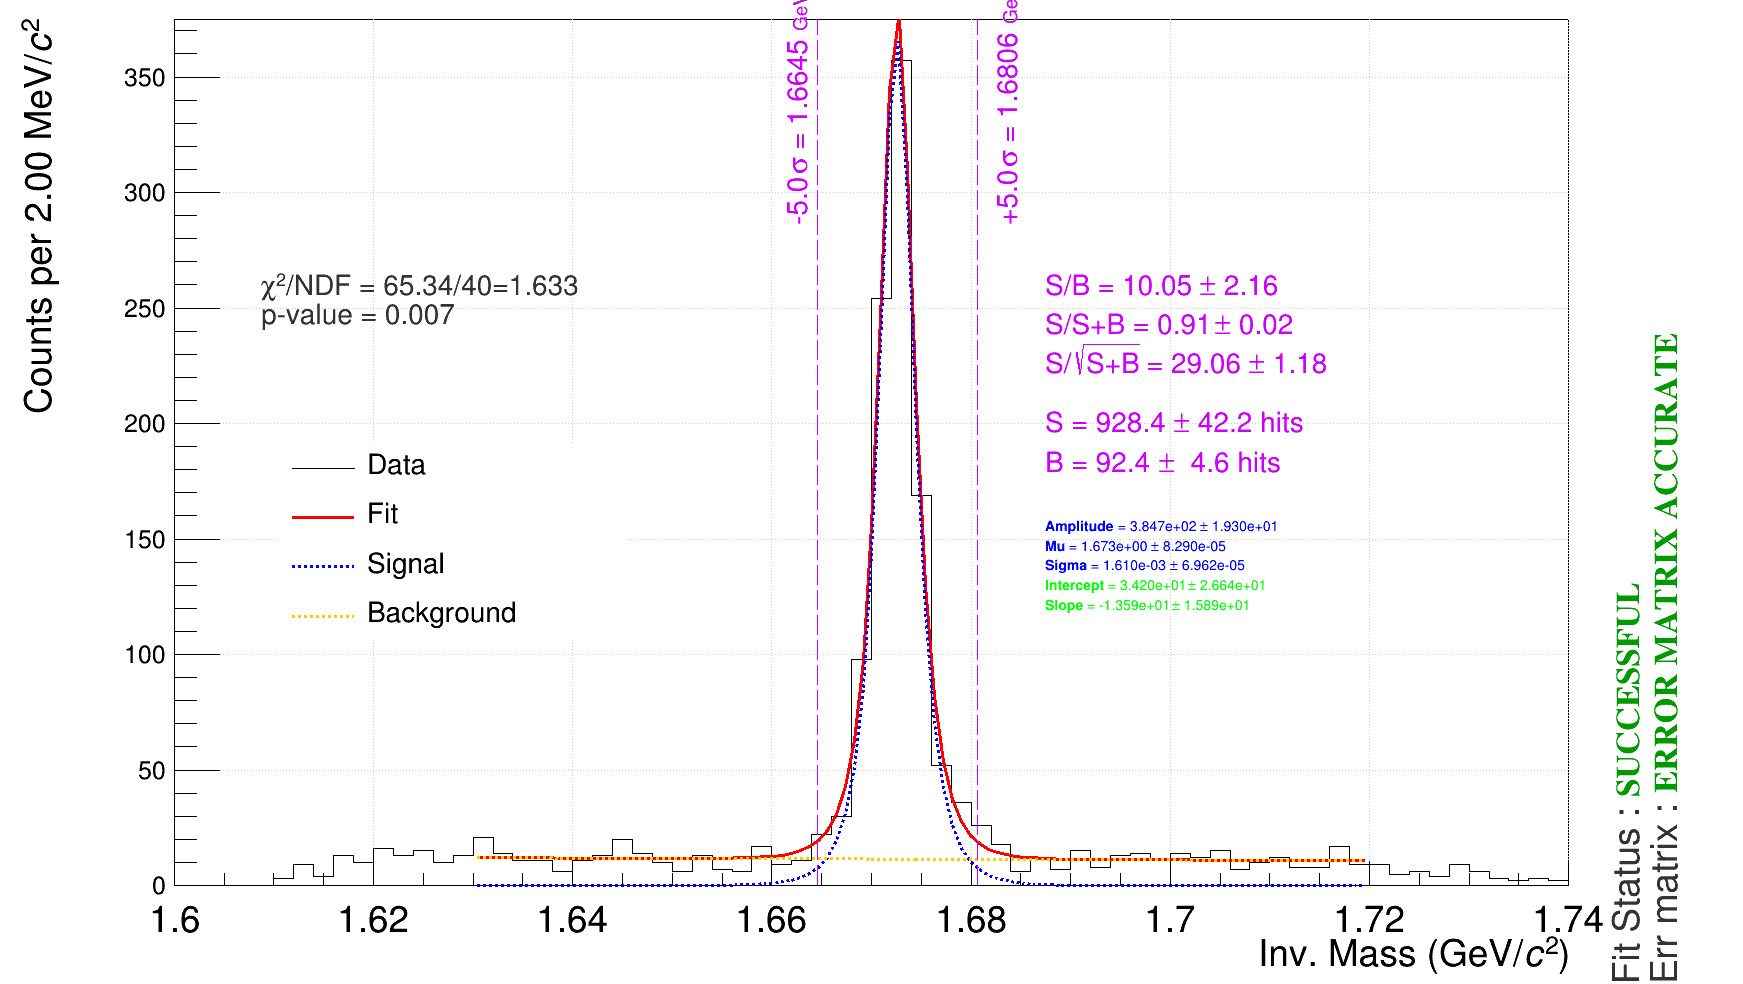
\includegraphics[width=1.00\textwidth, angle=0, clip=true, trim=0cm 0 0 0]{Figures/Sec04_TrackSelections/InvMassOmega.png} 
\caption{Invariant mass distribution for \rmOmega in multiplicity class I. The candidates are reconstructed in \absrap < 0.5. Blue dashed line represents the signal fit ; the region delimited by the two dashed purple lines defines the \textit{signal region}, used to extract raw signal of \rmOmega.}
\label{fig:InvMassOmega}
\end{figure}

\subsection{\rmPhiMes case}
\label{sec:Section04.b-}

\subsubsection{Candidate selections}

\rmPhiMes resonances are studied in the following decay channel :

\rmPhiMes [$s\bar{s}$] $\rightarrow$ \Kplus [$u\bar{s}$] \Kminus [$\bar{u} s$]  \qquad \textsc{B.R. 49.2 \%}

This resonance is reconstructed by forming pairs of tracks of opposite charge ; in the following, these pairs will be called "same-event pairs" . Due its short lifetime of 46.4 \fm \cite{noauthor_pdglive_nodate}, misassociations can not be discarded with a set of geometrical selections like in \rmOmega reconstruction, leading a large combinatorial background. This background is evaluated and then substracted using two techniques presented later in this section.

Tracks are being selected using standard ITS/TPC track cuts from 2011. High-quality tracks are ensured by restricting the number of crossed rows in TPC to be greater 70 (out of 159 pad rows) ; its ratio to the number of findable clusters should exceed 0.8. This is also achieved via cuts on $\chi^2$ per cluster. The latter  quantity on reconstructed tracks in the TPC and in the ITS are requiered to be smaller than 4 and 36 respectively ; $\chi^2$ value between TPC track constrained to the SPD vertex and global track must be inferior to 36. Only tracks following this requierements are retained : at least one hit in the innermost layer of the ITS, and the distance of closest approach to the primary vertex (DCA) lower than $0.0105 + 0.035 \pT^{-1.01}$ cm in the transverse plane and 2 cm along the longitudinal direction. In addition, kink decay topologies are discarded. This allows to reject secondary particles coming from weak decay. Each track has to lie in the pseudo-rapidity window \abspseudorap < 0.5 and to carry a transverse momentum between 0.15 and 4 \gmom. Energy loss in the TPC must be consistent with the PID hypothesis within $\pm$ 2 $\sigma$. If track matches a hit in the TOF, time of flight measurement is then used to select tracks compatible in $\pm$ 3 $\sigma$ with particle's species hypothesis.
Only resonance candidates sitting in the rapidity interval \absrap < 0.5 are selected. 

\begin{table}[h]
    \centering
    \begin{tabular}{c|c}
    \noalign{\smallskip}\hline \hline \noalign{\smallskip}
    \bf Track variable & Selections \rmPhiMes \\
    \noalign{\smallskip}\hline \hline \noalign{\smallskip}
    \pT interval (\gmom) & 0.15 < \pT < 4 \\
    Daughter pseudo-rapidity interval & \abspseudorap < 0.8 \\
    TPC $\text{d}E/\text{d}x$ & < 2 $\sigma$ \\    
    TOF $\beta$ (veto only) & < 3 $\sigma$ \\    
    \noalign{\smallskip}\hline \noalign{\smallskip}
    
    \multicolumn{2}{l}{\textbf{Standard ITS/TPC Cuts 2011}} \\
    ITS refit & \CheckGr \\
    TPC refit & \CheckGr \\
    Kink Topology & \NoWay \\
    Nbr of crossed rows & > 70 \\
    Nbr of crossed rows over findable clusters & $\geq$ 0.8 \\
	$\chi_\textsc{TPC}^2$ & < 4 \\
	$\chi_\textsc{TPC-CG}^2$ & < 36 \\
	$\chi_\textsc{ITS}^2$ & < 36 \\
	Nbr of clusters in SPD & $\geq$ 1 \\
	\textsc{DCA}xy (cm) & < 0.0105 + 0.035 \pT$^{-1.01}$ \\
	\textsc{DCA}z (cm) & < 2 \\
	DCAToVertex2D & \NoWay \\
	RequireSigmaToVertex & \NoWay \\
    \noalign{\smallskip}\hline \hline \noalign{\smallskip}
    \bf Candidate variable & Selections \rmPhiMes \\
    \noalign{\smallskip}\hline \hline \noalign{\smallskip}    
    Resonance rapidity interval & \absrap < 0.5 \\
    MC association (MC only) & Correct identity assumption on casc. and daughters \\ 
    \noalign{\smallskip}\hline \hline \noalign{\smallskip}
    \end{tabular}
    \caption{Summary of the track and candidate selections used for the reconstruction of \rmPhiMes.}\label{tab:PhiSel}
\end{table}

To tackle the combinatorial background, two approaches have been followed in this work. In the "mixed-events" method, each track from one event is paired with tracks of opposite charge coming from five different events in order to build uncorrelated pairs. Only the events whose difference in longitudinal position of primary vertex remains in $\pm$ 1 cm and multiplicity percentile, calculated from the V0M amplitude, coincides with $\pm$ 10\% are considered for the mixing. The mixed-event distribution is normalized by two times the number of mixed-events. In the second approach, one track from the resonance candidate (either the positive or the negative daughter) is rotated by 180 degree along the $z$ axis. Doing so, correlation between the two daughters is broken, leading to an uncorrelated pair. In this case, normalization factor is calculated such that the integral of the same-event and rotated-event distribution in the region 1.04 < $m_{KK}$ < 1.06 \gmass coincides. 

After normalization, the final invariant mass distribution is obtained by substraction of the same-event pair distribution by the uncorrelated pair distribution. In the following, the remaining background will be named \textit{residual background}.

\subsubsection{Raw signal extraction}

For each \pT bin, in the mass window 0.990 < $m_{KK}$ < 1.060 \gmass, signal peak is fitted by a Voigt function (convolution of Breit-Wigner, for the ideal signal, and a Gaussian, for detector resolution) added by a first order polynomial for the residual background. Raw signal is then extracted by the integral of the Voigt function within the fitting range.

\begin{equation}
\frac{\text{d}N}{\text{d}m_{KK}} = \frac{A \Gamma}{(2\pi)^{3/2} \sigma} \int\limits_{-\infty}^{\infty} \text{exp} \big [ -\frac{(m_{KK} - m')^2}{2\sigma^2} \big ] \frac{1}{(m' - \mu)^2 + \Gamma^2/4} \text{d} m'
\end{equation}\label{eq:PhiSignal}

Width of the \rmPhiMes is fixed to its nominal value $\Gamma$ = 4.29 \mev \cite{noauthor_pdglive_nodate}, and the resolution $\sigma$ is kept as a free parameter. \fig \ref{fig:InvMassPhi} illustrates an example of the invariant mass distribution obtained with the aforementionned procedure, on which a \rmPhiMes peak arises on top of a residual background. 

\begin{figure}[h]
	\centering
	\begin{subfigure}[b]{.45\linewidth}
         \centering
         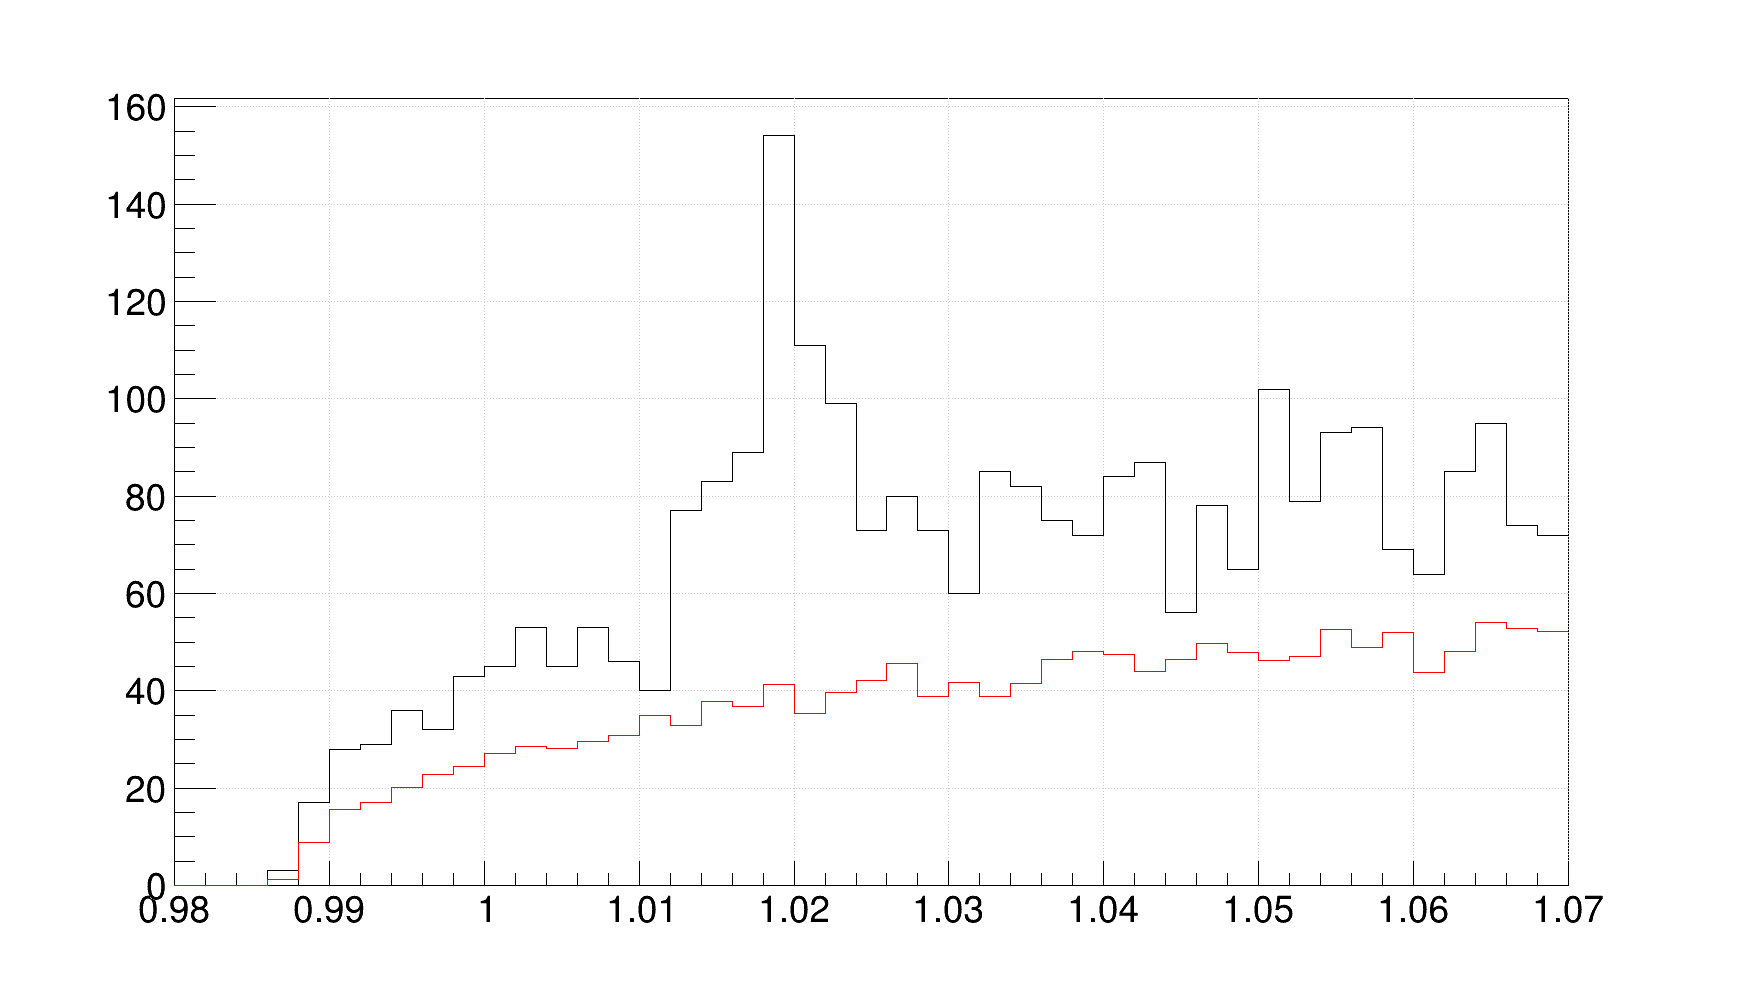
\includegraphics[width=1.2\textwidth, angle=0, clip=true, trim=0cm 0 0 0]{Figures/Sec04_TrackSelections/Phi+EvtMixing.png} 
         \caption{ }
         \label{fig:InvMassPhi+Mixed}
    \end{subfigure}
    \hfill
    \begin{subfigure}[b]{.45\linewidth}
         \centering
         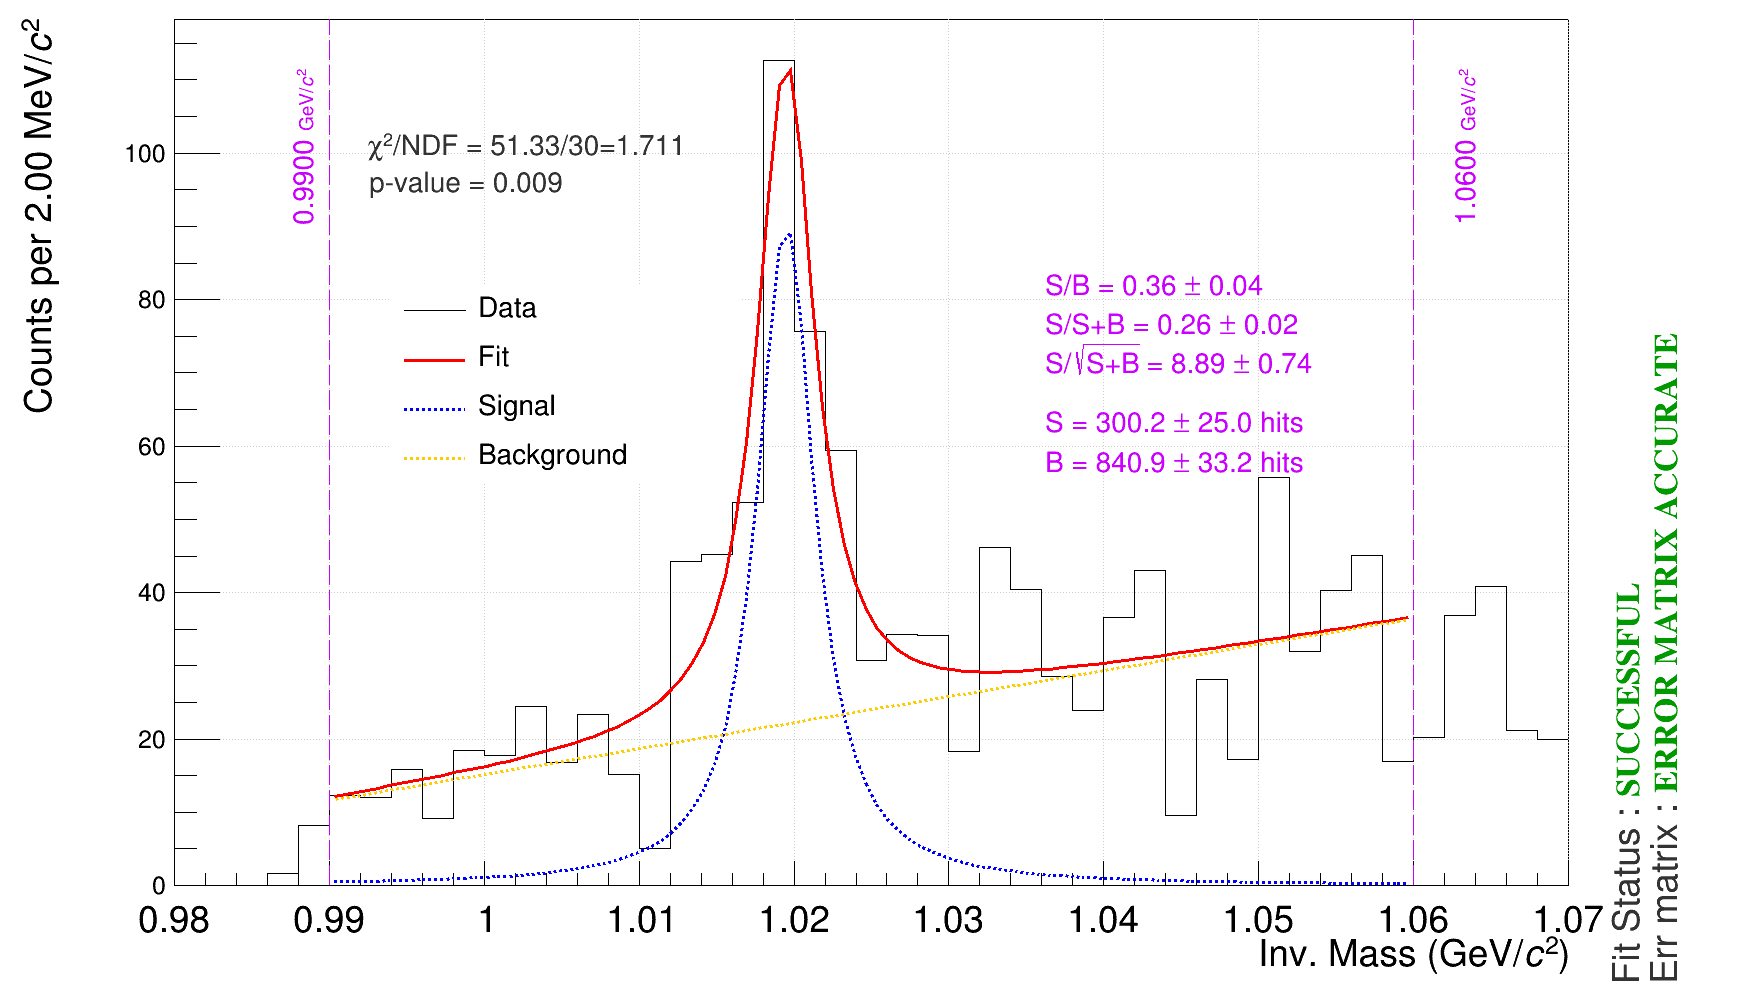
\includegraphics[width=1.1\textwidth, angle=0, clip=true, trim=0cm 0 0 0cm]{Figures/Sec04_TrackSelections/InvMassPhi.png}
         \caption{ }
         \label{fig:InvMassPhiSub} 
    \end{subfigure}
    \hfill
\caption{Invariant mass distributions for \rmPhiMes in multiplicity class I. The candidates are reconstructed in \absrap < 0.5. \fig \ref{fig:InvMassPhi+Mixed} : Same-event pairs distribution in black, normalized mixed-event pairs distribution in red. \fig \ref{fig:InvMassPhi} : Substraction of same-event and normalized mixed-pair distributions. Blue dashed line represents the signal fit ; the region delimited by the two dashed purple lines defines the \textit{signal region}, used to extract raw signal of \rmPhiMes.}
	\label{fig:InvMassPhi}
\end{figure}


\subsection{Yield extraction}
\label{sec:Section04.c-}

For each \pT bin, raw yield is calculated from the previously extracted raw signal using the expression \eq \ref{eq:RawYield} :
\begin{equation}
\frac{\text{d}^2 N}{\text{d}\pT \text{d} y} \bigg\rvert_\textsc{raw} = \frac{S_\text{raw}}{\Delta \pT \Delta y}
\end{equation}\label{eq:RawYield}

Raw particle yields are then corrected in acceptance (A) and efficiency ($\epsilon_\textsc{rec}$) using a MC data sample : the enriched one for the \rmOmega, and the general purpose one for the \rmPhiMes. The goal is to estimate the efficiency factor, $\epsilon$, in \eq \ref{eq:Efficiency}. The numerator corresponds to the number of reconstructed \rmOmega/\rmPhiMes; reconstruction is performed as if it would be real data, with an additionnal request : only reconstructed cascade/resonance associated to a generated \rmOmega/rmPhiMes are selected. This ensures the efficiency factor to be defined between 0 and 1. Denominator contains the number of generated particles in the selected events, coming directly from MC truth. To avoid bin flow effect, the same set of selection must be applied on both numerator and denominator ; this concerns the cuts on the rapidity and on the transverse momentum. \fig \ref{fig:EffOmega} and \ref{fig:EffPhi} show efficiency factors as a function of \pT, for \rmOmega and \rmPhiMes respectively.

\begin{equation}
\epsilon = A\times \epsilon_\textsc{rec} \times \text{B.R.} = \frac{\text{Number of reconstructed \hPM}}{\text{Number of generated \hPM}}
\end{equation}
\label{eq:Efficiency}

Once efficiency factors are evaluated for each \pT bin, corrected yields is given by dN/dptdy$|_\textsc{raw}/\epsilon$. Uncertainties on $\epsilon$ are not propagated, they will be included in the systematic uncertainties. Once the yield is extracted for each \pT bin, they are all summed and uncertainties are added in quadrature. 

\begin{figure}[h]
	\centering
	\begin{subfigure}[b]{.45\linewidth}
         \centering
         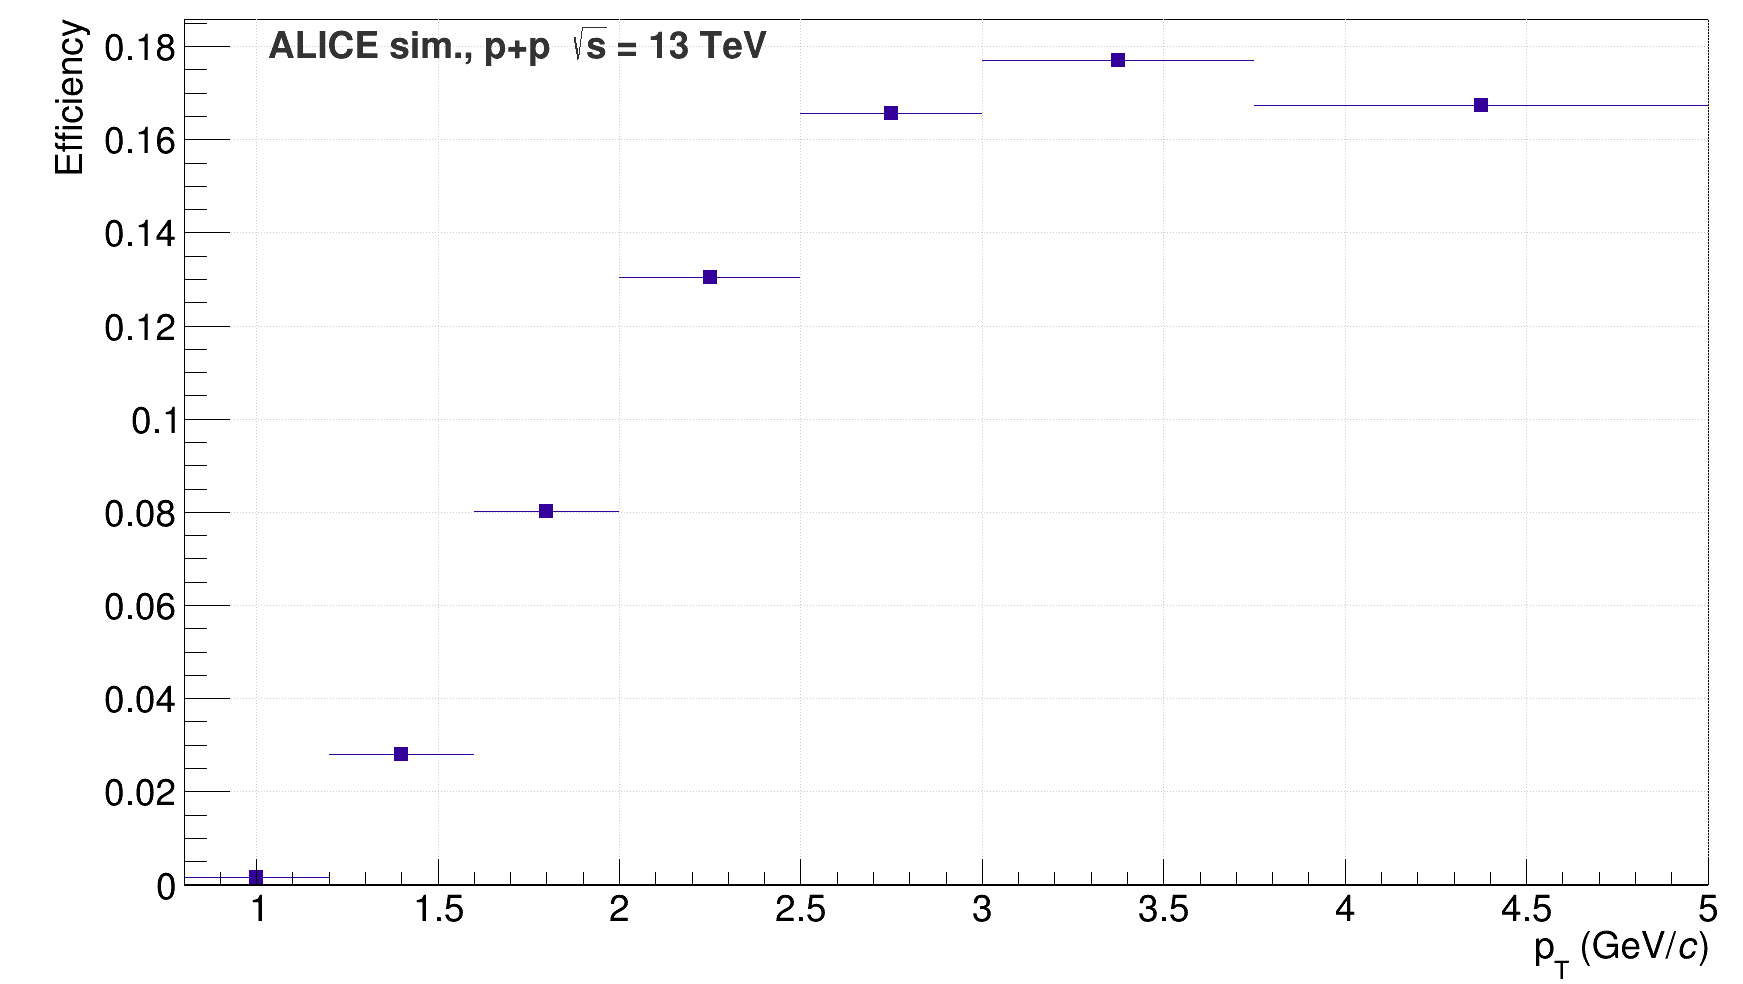
\includegraphics[width=1.\textwidth, angle=0, clip=true, trim=0cm 0 0 0]{Figures/Sec04_TrackSelections/EffOmega.png} 
         \caption{ }
         \label{fig:EffOmega}
    \end{subfigure}
    \hfill
    \begin{subfigure}[b]{.45\linewidth}
         \centering
         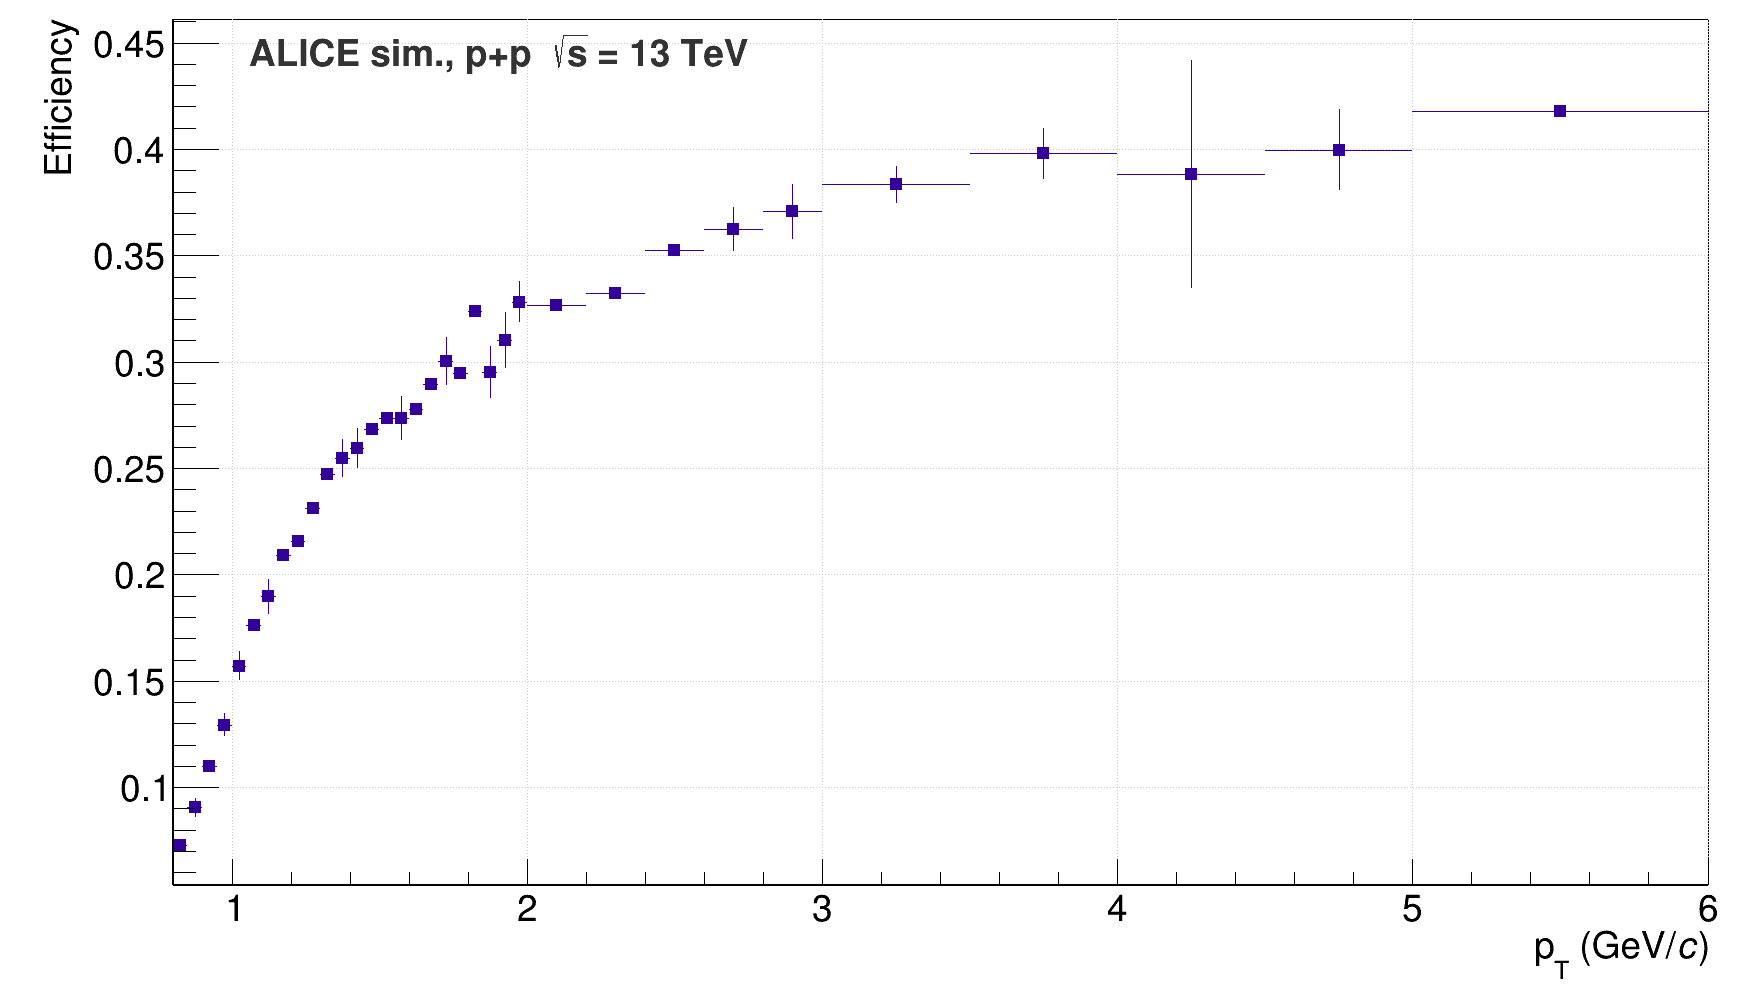
\includegraphics[width=1.\textwidth, angle=0, clip=true, trim=0cm 0 0 0cm]{Figures/Sec04_TrackSelections/EffPhi.png}
         \caption{ }
         \label{fig:EffPhi} 
    \end{subfigure}
    \hfill
\caption{Efficiency factors as a function of \pT for \ref{fig:EffOmega}) \rmOmega and \ref{fig:EffPhi}) \rmPhiMes . Efficiency factor is integrated in multiplicity of the event and in rapidity of the candidates. The candidates are reconstructed in \absrap < 0.5. \fig \ref{fig:EffOmega} has been obtained with the MC sample enriched in \rmXis and \rmOmegas ; \fig \ref{fig:EffPhi} has been extracted using five runs of the general purpose MC. }
	\label{fig:Eff}
\end{figure}

Following the prediction to be tested, only events presenting at least one \rmPhiMes resonance should be selected, and \rmOmega yield should be extracted afterwards. As a matter of fact, it is completely equivalent to do the opposite, meaning : filter events with at least one \rmOmega, and then extract \rmPhiMes yield. However, it has been shown, in sections \ref{sec:Section04.a-} and \ref{sec:Section04.b-}, that both species have distinct purities. Consequently, even if the two approaches of the \Pythiaeight prediction are equivalent, one may introduce more noise than the other. With a purity exceeding 90\%, the second approach appears to be the most strategic choice. 
